%\documentclass[12pt, letterpaper, titlepage]{article}
\documentclass[12pt, letterpaper]{article}

\usepackage{amsmath, amsfonts}
\usepackage{booktabs}
\usepackage{amsthm}
\usepackage{graphicx}
\usepackage[margin=1in]{geometry}
\usepackage{hyperref}
\usepackage{cleveref}
\hypersetup{colorlinks = true, linkcolor = blue, citecolor=blue, urlcolor = blue}
\usepackage{natbib}
\usepackage{float}
\usepackage{setspace}
\usepackage{pdfpages}
\usepackage{lineno}
\usepackage{mwe}
\usepackage{comment}
\linenumbers*[1]
% %% patches to make lineno work better with amsmath
\newcommand*\patchAmsMathEnvironmentForLineno[1]{%
 \expandafter\let\csname old#1\expandafter\endcsname\csname #1\endcsname
 \expandafter\let\csname oldend#1\expandafter\endcsname\csname end#1\endcsname
 \renewenvironment{#1}%
 {\linenomath\csname old#1\endcsname}%
 {\csname oldend#1\endcsname\endlinenomath}}%
\newcommand*\patchBothAmsMathEnvironmentsForLineno[1]{%
 \patchAmsMathEnvironmentForLineno{#1}%
 \patchAmsMathEnvironmentForLineno{#1*}}%

\AtBeginDocument{%
 \patchBothAmsMathEnvironmentsForLineno{equation}%
 \patchBothAmsMathEnvironmentsForLineno{align}%
 \patchBothAmsMathEnvironmentsForLineno{flalign}%
 \patchBothAmsMathEnvironmentsForLineno{alignat}%
 \patchBothAmsMathEnvironmentsForLineno{gather}%
 \patchBothAmsMathEnvironmentsForLineno{multline}%
}

% control floats
\renewcommand\floatpagefraction{.9}
\renewcommand\topfraction{.9}
\renewcommand\bottomfraction{.9}
\renewcommand\textfraction{.1}
\setcounter{totalnumber}{50}
\setcounter{topnumber}{50}
\setcounter{bottomnumber}{50}

\newcommand{\jy}[1]{\textcolor{blue}{JY: #1}}
\newcommand{\eds}[1]{\textcolor{red}{EDS: (#1)}}
\newcommand{\of}[1]{\textcolor{violet}{OF: #1}}

% NOTE: To produce blinded version, replace "0" with "1" below.
\newcommand{\blind}{0}

%\title{On Devon Allen's Disqualification at the 2022 World Track and Field 
%Championships} 
%
%\author{Owen Fiore\\
%%   \href{mailto:owen.fiore@uconn.edu}
%% {\nolinkurl{owen.fiore@uconn.edu}}\\
  %Elizabeth D. Schifano\\
  %Jun Yan\\[1ex]
  %Department of Statistics, University of Connecticut\\
%}
%\date{}

\begin{document}
%\maketitle

\if0\blind
{
  \title{\bf On Devon Allen's Disqualification at the 2022 World Track and Field 
Championships}
  \author{Owen Fiore, %\\
%   \href{mailto:owen.fiore@uconn.edu}
% {\nolinkurl{owen.fiore@uconn.edu}}\\
  Elizabeth D. Schifano, %\\
  Jun Yan\\[1ex]
  Department of Statistics, University of Connecticut\\
}
\date{}
  \maketitle
} \fi

\if1\blind
{
  \bigskip
  \bigskip
  \bigskip
  \begin{center}
  {\LARGE\bf On Devon Allen's Disqualification at the 2022 World Track and Field 
Championships}
\end{center}
  \bigskip
} \fi


\doublespace

% Abstract should be under 200 words

\begin{abstract}
Devon Allen was disqualified from the men's 110-meter hurdle final at
the 2022 World Track and Field Championships after recording a
reaction time of 0.099 seconds—just 0.001 seconds faster than the
allowable threshold of 0.1 seconds. This paper explores whether the
reaction times of athletes at the 2022 Championships were unusually
fast compared to other competitions and evaluates the appropriateness
of the 0.1-second disqualification barrier. To investigate these
issues, we employ a rank-sum test for clustered data to compare
athletes' reaction times across multiple competitions, along with a
generalized linear mixed model (GLMM) that accounts for both venue and
heat effects. The results indicate that athletes at the 2022
Championships had significantly faster reaction times on average. This
analysis raises important questions about the validity of the current
reaction time threshold and suggests potential modifications to the
rules that could prevent future disqualifications under similar
circumstances.


\bigskip\noindent{\sc Keywords}:
False Start, GLMM, Hurdle, Reaction Time, Seiko, rank-based test

\end{abstract}

\doublespace


\section{Introduction}
\label{sec:intro}

Devon Allen’s highly anticipated performance at the 2022 World 
Track and Field Championships in Eugene, Oregon, ended in 
controversy when he was disqualified for a reaction time of 
0.099 seconds, just 0.001 seconds below the allowable threshold.
Allen, a University of Oregon alumnus, 
had recently run a time of 12.84 seconds in the 110-meter hurdle 
event, just 0.04 seconds short of the world record. After placing 
third at the U.S. Track and Field Championships, he advanced 
through the preliminary heats and semifinals at the World 
Championships, with reaction times of 0.123 and 0.101 seconds, 
respectively. However, in the final heat, competing in front of his 
home audience, Allen’s reaction time was just 0.001 seconds faster 
than the 0.1-second threshold set by the International Association 
of Athletics Federations (IAAF), resulting in his disqualification, a 
decision that was met with widespread public outcry.


The disqualification of Allen was widely discussed in online 
communities, with some questioning the accuracy of the timing 
equipment. One of the most active platforms was \url{www.LetsRun.com}, 
a website that functions as both a message board and a news outlet. 
The message board, similar to Reddit, is particularly active during 
major running events, including the Olympics and the World Track 
and Field Championships. The news section of the website featured 
articles such as \citep{johnson2022data} and \citep{johnson2022was} 
by Robert Johnson, the site’s founder. Johnson argued that there may 
have been an error with the timing equipment at the 2022 Championships. 
He cited graphs and descriptive statistics, like median reaction 
times, comparing the reaction times at the 2022 Championships to 
those from other competitions, including the U.S. Championships and 
previous World Championships. However, these comparisons lacked formal 
statistical analysis. 


The 0.1-second disqualification threshold in track events has been 
a subject of ongoing debate, with researchers presenting evidence 
both in favor of lowering and raising the
limit. \citet{pain2007sprint} examined
reaction times in nine male athletes and found that the fastest athlete 
had an average reaction time of 0.087 seconds, with a standard deviation 
of 0.004 seconds. Similarly, \citet{komi2009iaaf}, in a study commissioned 
by the IAAF, recommended lowering the disqualification threshold to 0.08 
or 0.085 seconds, arguing that athletes are capable of faster reaction 
times than the current threshold allows. On the other hand, some 
researchers have argued for increasing the threshold.
\citet{brosnan2017effects} suggested raising it to 0.115 seconds based
on data from European and World Championships, while a study of the
2008 Olympics supported the conclusion that athletes cannot reliably
react within 0.1 seconds \citep{lipps2011implications}. Interestingly,
\citet{brosnan2017effects} and \citet{lipps2011implications} relied on
retrospective event data, whereas \citet{pain2007sprint} and
\citet{komi2009iaaf} conducted controlled experiments to assess
reaction time capabilities. The IAAF has not revised the threshold
since its implementation in 1999.


This paper has two primary objectives. First, we investigate whether 
reaction times at the 2022 World Championships were significantly 
different from other competitions, focusing on athletes who competed 
in multiple events. Using a matched-pairs design, we compare reaction 
times across the 2022, 2019, and 2023 World Championships, as well as 
the 2022 national-level competitions. This approach isolates the 
effect of the competition year while controlling for individual 
performance. The second objective is to assess the 
appropriateness of the 0.1-second threshold by modeling reaction 
times from World Championships held from 1999 onward. We use a gamma 
linear mixed-effects model with random effects for both venue and heat. 
This model estimates the probability of reaction times falling below 
the threshold, helping evaluate the consistency of reaction times and 
whether the current threshold is statistically justified.


The rest of this paper is organized as follows. Section~\ref{sec:Data} 
describes how the data were collected. The rank-sum test, detailed 
in Section~\ref{sec:rank}, uses slightly different data from the 
generalized linear mixed-effects model (GLMM) developed in 
Section~\ref{sec:glmm}. Section~\ref{sec:Results} presents the results 
of both analyses and discusses the implications of the reaction time 
barrier. Finally, Section~\ref{sec:concludingremarks} outlines the 
paper’s impact and limitations. All data and code for our analysis 
are provided in the supplementary materials.


\section{Data} \label{sec:Data}

There are two types of data that are explored throughout this paper. For the
rank-sum tests described in Section~\ref{sec:rank}, the data comes from male 
athletes who competed in the 110 meter hurdles and 100 meter dash, and female
athletes who competed 100 meter hurdles and 100 meter dash.
Athletes must have competed in the 2022 World Championships and another competition 
(2019 World Championships, 2023 World Championships, or 2022 national 
championships). For the GLMM described in Section~\ref{sec:glmm}, data comes
from every world championships from 1999 to 2023 and includes reaction times from
the 110 meter hurdles and 100 meter dash. This investigation started 
shortly after the 2022 World Championships, but as the 2023 data has now become 
available, we are pleased to include it in both of our analyses, and it did not
significantly change our results \citep{WAData}. 


\subsection{Comparison Data with 2022 World Championships}
\label{sec:databeyond}

The motivation for looking beyond World Championships data came from an 
exploratory analysis examining how United States athletes reacted at the 
2022 United States Track and Field Championships.


\subsubsection{2022 National Competitions}\label{sec:datanational}
From June 23-26, 2022, the United States held its Track and Field Championships 
at Hayward Field in Eugene, Oregon to decide who to send to the World 
Championships being held at the same venue in August. Thus, we can establish a 
baseline for the four United States athletes who competed in at least one round 
of both events: Trey Cunningham, Daniel Roberts, Grant Holloway, and Devon Allen.  
Every athlete reacted faster in all the World Track and Field Championships 
races compared to the United States Track and Field Championships races. The 
dataset of the four United States athletes is too small to perform any 
meaningful statistical analysis, but the data was expanded to include reaction 
times from more athletes who competed at other national competitions (many of which were 
held from May-July of 2022). This data was difficult to find, as the data is not
centrally located but instead found on different national websites (often 
recorded in the national language without translation).


Each athlete was designated as a ``cluster'' and the stage of competition (national
or international) was specified for each competition within the cluster (athlete).
Thus, this is subunit level grouping where we assign the treatment, national or
international, within each cluster. Cluster sizes range from three to six, with
one cluster of size three, six clusters of size four, two clusters of size five,
and two clusters of size six.
\of{This explanation is going to need to be re-worked now that we have more data.
Should we make a table of some sort? It's going to be very wordy without one}

We chose to include preliminary rounds in this section as well as in
Section~\ref{sec:data2019}, as removing them would have resulted in a much
narrower analysis with fewer athletes and clusters.


\subsubsection{Other World Track and Field Championships}\label{sec:data2019}
The 2019 and 2023 World Track and Field Championships data is included in the 
larger dataset described in Section~\ref{sec:dataworld}, but we can also use it
similarly to how we used national level in Section~\ref{sec:datanational}. We
can compare the times of athletes who participated in the 2022 Championships with
their times at another World Championships: 2019 and/or 2023.


While it is theoretically possible that athletes got faster 
between 2019 and 2022 or 2022 and 2023, it is important to 
remember that these are some of the fastest sprinters on the planet, and thus
improving on elite times is not easy. Once again we repeat a similar procedure
as in Section~\ref{sec:datanational}; we assign each athlete to be a cluster and
within each cluster label times to be from either the 2019, 2022, or 2023 World
Championships. When comparing 2019 and 2022 we look at data from 15
athletes, with two clusters of size two, three clusters of size three, five 
clusters of size four, two clusters of size five, and three clusters of size six.
When comparing 2022 and 2023 we look at data from 22 athletes, with seven 
clusters of size two, three clusters of size three, six clusters of size four,
and six clusters of size five.
\of{This explanation might need to change}

\begin{figure}[tbp]
  \centering
  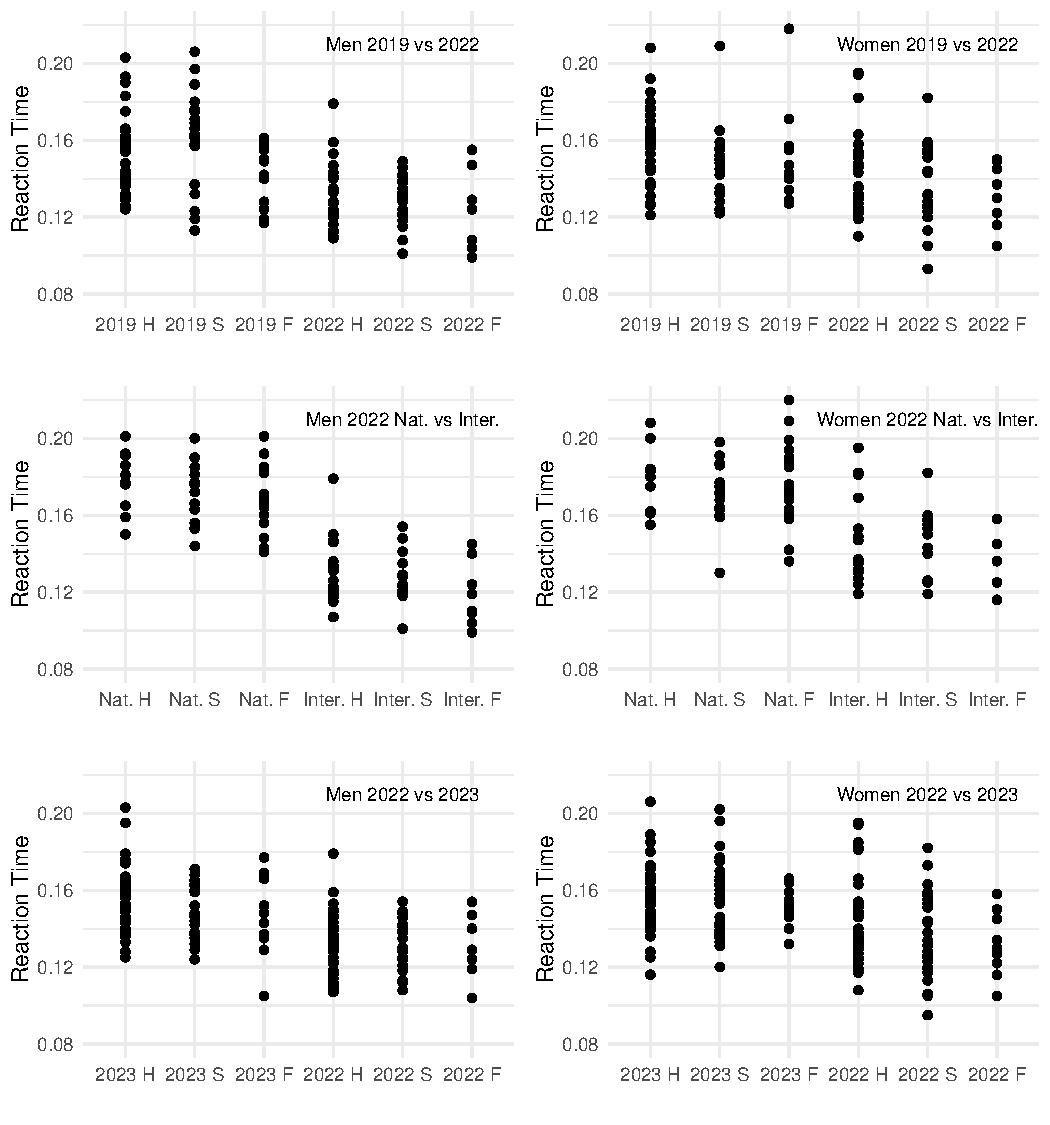
\includegraphics{RankScatterPlots}
  \caption{This collection of scatterplots of data used in the rank comparison
  section shows that times in 2022 were on average lower. On the horizontal
  axis below each graph "H", "S", and "F" refer to the heats, semifinals, and 
  finals respectively. Please note that in the last row the 2022 times are to
  the right of the 2023 times.}
  \label{fig:RankScatterplots}
\end{figure}

Figure~\ref{fig:RankScatterplots} shows the data that will be analyzed
with the rank-based methods (described in Section~\ref{sec:rank} with results in 
Section~\ref{subsec:Results_Rank}). In each of the six graphs, the reaction 
times for athletes who competed at the 2022 World Championships
are compared to their reaction times at another at which they competed. 
It is worth noting that each instance of the 2022 data is different, because
those who competed at both the 2019 and 2022 World Championships will be
different athletes than those who competed at both the 2022 and 2023 World
Championships. This data was only for athletes who competed
in at least one race at each championship, however it is possible for athletes
to have competed in one race in 2019 and two races in 2022. The 2022 World
Championship heats and semifinals both had on average lower reaction times than
their respective other (2019, 2023 or 2022 national) races, and the 2022 World 
Championship finals were substantially faster.  It
is also worth noting is that the fastest reaction time in the 2022 World
Championships Finals and Semifinals both came from Devon Allen, but the 
difference between 0.101 and 0.099
seconds was the difference in what caused him to be disqualified. 


\subsection{World Championships 1999--2023}\label{sec:dataworld}


Data was taken from the World Athletics 
and covers the men's 110 meter hurdles from 1999 to 2023.
We focus on the reaction times during the 
semifinal and final heats only, as reaction times from preliminary heats are 
often not as fast as those in later heats \citep[e.g.,][]{zhang2021correlation}. 
For analysis purposes, we will pool reaction times of men's final and 
men's semifinal heats together which increases the sample size. This is 
advantageous because in some years there are very few finals observations, such
as in 2022, when there were only five data points due to two disqualifications 
and one athlete who did not compete. This is the data that we will reference
throughout the rest of the paper unless otherwise noted. We also consider data 
that excludes 2022 to see how our analysis differs based on the exclusion of one
particular year of interest.


The data under consideration is summarized using side-by-side boxplots in 
Figure~\ref{fig:Boxplot}. It is clear that the reaction times in the 2022
boxplot are lower (indicating faster reaction times) than in many of the other
years. The median reaction time in 2022 was 0.129 seconds,  compared to 0.156
seconds, which is what \citet{brosnan2017effects} found when looking at data
from 1999 to 2014. We can also see from Figure~\ref{fig:Boxplot} that the 
reaction times clearly differ from year to year. The venue of the World 
Championships changes each year, so weather or climate related factors such as 
humidity, precipitation, elevation, may indeed play a role, but additionally,
both the technology and false start penalization rules have changed over the 
study period.


\begin{figure}[tbp]
  \centering
  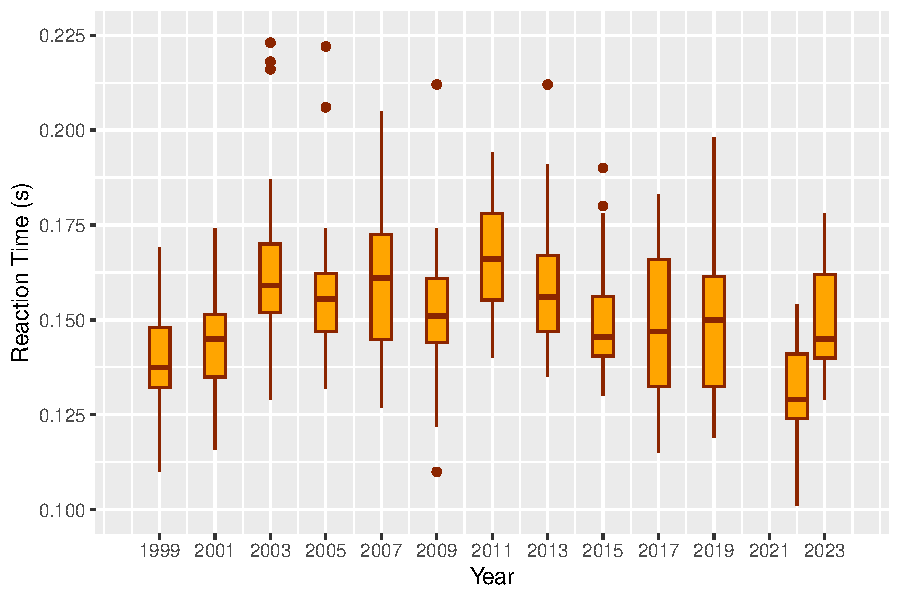
\includegraphics{Boxplot}
  \caption{The reaction times from 1999 to 2023 for the men's 110 meter hurdle
  and 100 meter dash.}
  \label{fig:Boxplot}
\end{figure}
\of{Do We want 2 boxplot figures: 1 hurdles, 1 dash or combine them}

From 2007 to 2009, the IAAF (the former name for World Athletics, and the 
governing body for the World Track and Field Championships) instituted a rule 
change that allowed one warning false start before a sprinter was disqualified 
\citep{iaaf2009falsestart}. There were 18 male and 7 female false starts at the 
2007 World Championships, and 18 male and 7 female false starts at the 2009 World 
Championships. Starting in 2011, the rule was scrapped, and the old policy which
automatically disqualifies runners who false start was reinstated. This was 
desirable for World Athletics as false starts can make already lengthy track 
meets more tedious, both for athletes and viewers watching the television 
broadcast. By returning to the harsher policy and cracking down on false starts,
World Athletics had reduced men's false starts by two thirds in 2011 (6 male and
4 female disqualifications) \citep{iaaf2009falsestart}. \citet{haugen2013effect}
examined the effect of different false start rules that IAAF has imposed from 
1997 to 2009 and found statistically significant improvement in reaction times 
under more lenient rules.



\section{Methods} \label{sec:Methods}

The data described in Sections~\ref{sec:databeyond} and~\ref{sec:dataworld} were
analyzed with rank-based methods and a GAMLSS, respectively.


\subsection{Rank-based Comparison}\label{sec:rank}


To test the conjecture that the 2022 World Championships timing device may have 
led to faster recorded reaction times, we compare the reaction times of the same
athletes who have attended both the 2022 World Championships and other 
competitions. 
In this setting, we have clustered data with subunit grouping. In particular,
each athlete is a cluster and the multiple reaction times from the same athlete
can be from either the 2022 World Championships or otherwise.
Let $X_{ij}$ be the $j$th reaction time of athlete~$i$, $i = 1, \ldots, n$,
$j = 1, \ldots, m_i$ where $m_i$ is the number of observations from
athlete~$i$. Let $\delta_{ij}$ be the group indicator of $X_{ij}$; $\delta_{ij}
= 1$ if $X_{ij}$ is in group~1 (2022 World Championships) and $\delta_{ij} = 0$ 
otherwise. Athletes are
assumed to be independent, while subunit observations from the same athlete are
not. The null hypothesis $H_0$ to be tested is that there is no difference
between the two groups; i.e., the distribution of $X_{ij}$ remains the same
regardless of the group indicator $\delta_{ij}$.


\citet{datta2005rank} proposed an extension of the Wilcoxon rank-sum test to
clustered data with subunit-level grouping. The test is designed based on a
within-cluster resampling principle. Consider randomly picking one observation
from each cluster to form a pseudo-sample. Let $X_i^*$ be a random pick from the
$i$th cluster in the pseudo-sample and $\delta_i^*$ its group indicator. The
Wilcoxon rank-sum statistic for the pseudo-sample is
\[
W^* = \frac{1}{n + 1} + \sum_{i=1}^{n} \delta_{i}^{*} R_{i}^{*},
\]
where $R_{i}^{*}$ is the rank of $X_{i}^{*}$ in the pseudo-sample.
The test statistic $S$ is the average of $W^*$ averaged over all possible
pseudo-samples conditioning on the observed data and group indicators.
The mean and variance of $S$ under $H_0$ can be derived so that $S$ can be
standardized to form a $Z$ statistic which follows a standard normal distribution
asymptotically \citep[p.910]{datta2005rank}.


With our small sample size, the asymptotic normal distribution may not be
reliable, so we also use 1~million random permutations to simulate the null 
distribution of the test statistic.
This method is available from the \texttt{clusWilcox.test()} function
with \texttt{method = `ds'} (for \underline{D}atta and \underline{S}atten) and 
\texttt{exact = TRUE} from R package
\texttt{clusrank} \citep{jiang2020wilcoxon}. 


\subsection{GAMLSS}\label{sec:glmm}

Based on an exploratory analysis, the reaction times are adequately
modeled by a Generalized Gamma (GG) distribution with random effects in
model parameters. The GG distribution has three parameters, denoted by
$\text{GG}(\mu, \sigma, \nu)$ has density function
\[
f_Y(y \mid \mu, \sigma, \nu) = 
\frac{|\nu| \theta^\theta}{\Gamma(\theta) y} 
z^{\theta} \exp\left(-z \theta\right),
\]

for $y > 0$, $\mu > 0$, $\sigma > 0$, and $\nu \neq 0$,
where $z = \left(\frac{y}{\mu}\right)^\nu$,
$\theta = 1 / (\sigma^2 \nu^2)$.
$\Gamma(\cdot)$ denotes the Gamma function.
The GG distribution is highly flexible, encompassing several  
well-known distributions as special cases, such as the
Weibull ($\mu = \nu)$ and  Gamma $(\nu = 1)$ distributions.
Its mean is
$\mu \frac{\Gamma(\theta + 1 / \nu)}{\theta^{1 / \nu} \Gamma(\theta)}$,
provided $\theta > -1 / \nu$. Here,
$\mu$ scales the central tendency, $\sigma$ controls 
dispersion, and $\nu$ determines skewness. This parameterization allows 
the distribution to model asymmetric and heavy-tailed data effectively, making 
it particularly suitable for reaction times.
An implementation of this distribution is available from R package
\texttt{gamlss.dist} \citep{rigby2019distributions}.



Let $Y_{ijk}$ denote the reaction time of observation~$k$ in heat~$j$
of year~$i$. Conditioning on a venue effect $v_i$ for year~$i$ 
and a heat effect $h_{i/j}$ nested within each year~$i$, the
distribution of $Y_{ijk}$ is
$\text{GG}(\mu_{ijk}, \sigma_{ijk}, \nu)$, where
\begin{align}
\log(\mu_{ijk}) &= \beta_0 + v_i ,\\
\log(\sigma_{ijk}) &= \gamma_0 + h_{i/j},
\end{align}
$v_i$ is normally distributed with mean zero and
variance~$\sigma_v^2$, and $h_{i/j}$ is normally distributed with mean
zero and variance~$\sigma_h^2$.
The two random effects were found useful: one capturing the venue effect, which
is used to contrast years, and the second being the heat effect, where every
race was given a unique identifier with typically five to nine observations
per race. The heat effect is important as it captures the variability in the
amount of time athletes are on the starting blocks before the gun goes off.
This model can be fit with R package \texttt{gamlss}
\citep{stasinopoulos2024generalized}.


Model diagnosis and tail analysis can be done with the fitted GG model
from package \texttt{gamlss}. Normalized quantile residuals, or
z-scores \citep{dunn1996randomized}, of the observations can be
extracted with the \texttt{residuals} method of a \texttt{gamlss}
object. The z-scores can then be checked with a Q-Q plot
\citep{almeida2018ggplot2}. The marginal
distribution of $Y_{ijk}$ is a scale-mixture of GG distributions, which can be
easily simulated from once the parameters are estimated. Many
random numbers generated from the fitted mixture distribution can be used to
approximate the probability of observing a reaction time faster than any given
threshold. We are specifically interested in the probability of a reaction time
being less than 0.1 seconds in order to gauge if that is a reasonable 
disqualification barrier.



\section{Results} \label{sec:Results}

\subsection{Rank-based Comparison} \label{subsec:Results_Rank}

The rank-based methods described in Section~\ref{sec:rank} are used
to determine if the reaction times for athletes who had competed at other 
championships differed significantly from the 2022 World Championships. This is
a two group comparison performed three times: comparing 2019 and 2022 World
Championships, comparing 2022 and 2023 World Championships, and comparing 2022 
national championships to the 2022 World Championships.


\begin{table}
  \centering
  \caption{2019 vs 2022 compares data from the same athletes who competed at the
  2019 and 2022 World Track and Field Championships. 2022 vs 2023 compares data
  from the same athletes who competed at the 2022 and 2023 World Track and Field
  Championships. National vs International compares data from the same athletes
  who competed at 2022 national-level championships and the 2022 World Track and
  Field Championships.}
  \begin{tabular}{c c c c c} 
   \toprule
   Comparison & Permutation & Asymptotic & Athletes & Number observations  \\ 
   \midrule
   2019 vs 2022 Men & $2.8 \cdot 10^{-5}$ & $1.1 \cdot 10^{-5}$ & 34 & 134 \\
   2019 vs 2022 Female & $ 1.5 \cdot 10^{-3}$ & $6.9 \cdot 10^{-3}$ & 31 & 124 \\
   2022 Nat. vs Inter. Men & $<0.001$ & $ 6.1 \cdot 10^{-5}$ & 17 & 80 \\
   2022 Nat. vs Inter. Women & $<0.001$ & $ 1.2 \cdot 10^{-3}$ & 17 & 80 \\
   2022 vs 2023 Men & $<0.001$ & $1.4 \cdot 10^{-6}$ & 45 & 161 \\
   2022 vs 2023 Female & $<0.001$ & $9.4 \cdot 10^{-7}$ & 47 & 182 \\
   \bottomrule
  \end{tabular}
  \label{tab:Clusrankresults}
\end{table}
\of{Table might still be too wide.  I used <0.001 becuase that is what we
had currently been using for any values from the permutation test where the value
was < 2.2e-16 in R.  Professor Yan will know best, but are the sample sizes now
sufficiently large enough that the permutation test is not needed? If I recall
correctlty that was a correction for small sample sizes.}

Table~\ref{tab:Clusrankresults} shows the results generated from both the 
permutation and asymptotic rank-based tests for the six comparisons, 
as discussed previously in Section~\ref{sec:rank}. The national versus international
comparisons produced lower p-values than the 2019 versus 2022 and 2022 versus 2023
comparisons. The highly significant permutation test results
provides substantial evidence that both men and women who competed at the
2022 World Track and Field Championships were on average, significantly faster
at reacting than they were just a few months prior. When looked at in context
with other tests, these results show that athletes competing at the 2022 World
Track and Field Championships had faster reaction times than when they had
competed at other competitions.


\subsection{GLMM} \label{subsec:Results_GLMM}

\begin{table}
  \centering
  \caption{AIC and estimated parameters for the three models fitted to the
    data.}
  \label{tab:Gamma_parameters}
  \begin{tabular}{c c c c c c c}
    \toprule
    Data set & Model & AIC & $\sigma_h$ & $\sigma_v$ & $\alpha$ & $\sqrt{\phi}$ \\
    \midrule
    Excluding 2022 &
      Venue Effect Only & $-1862.2$ &   & 0.048 & $-1.857$ & 0.152\\
     & Heat Effect Only & $-1910.9$ & 0.069 &  & $-1.877$ & 0.136\\
     & Venue and Heat Effect & $-1912.9$ & 0.058 & 0.033 & $-1.868$ & 0.136\\[1ex]
    Including 2022 &
    Venue Effect Only & $-3798.8$ &   & 0.054 & $-1.871$ & 0.149\\
    & Heat Effect Only & $-2070.7$ & 0.073 &  & $-1.890$ & 0.135\\
    & Venue and Heat Effect & $-2075.7$ & 0.057 & 0.040 & $-1.881$ & 0.134\\
    \bottomrule
  \end{tabular}
\end{table}
\of{needs to be updated with current values. But I did start to alter something
then stopped.}

The estimated parameters of the GLMM model under the log link are shown in 
Table~\ref{tab:Gamma_parameters}, both excluding and including 2022 data.
Three models were considered, differing in their random effects: venue effect
only; heat effect only, and both venue and heat effects. Reported are the AIC
and estimated model parameters: the standard deviation
of the heat effect $\sigma_h$, the standard deviation of the venue
effect~$\sigma_v$, the intercept~$\alpha$, and the
square root of the dispersion parameter $\phi$. With or without 2022,
the GLMM with both venue and heat random effects was the best model as evidenced
by the AIC compared to the other models with only one random
effect.  When we exclude 2022 from the full model, we observe small but intriguing
discrepancies in the models. The standard deviation of the venue effect, 
$\sigma_v$, increases from 0.33 to 0.40 when 2022 is included, however, the
estimates of other parameters
remained relatively similar, such as the standard deviation of the heat effect
and the dispersion parameter.


\begin{figure}[tbp]
  \centering
  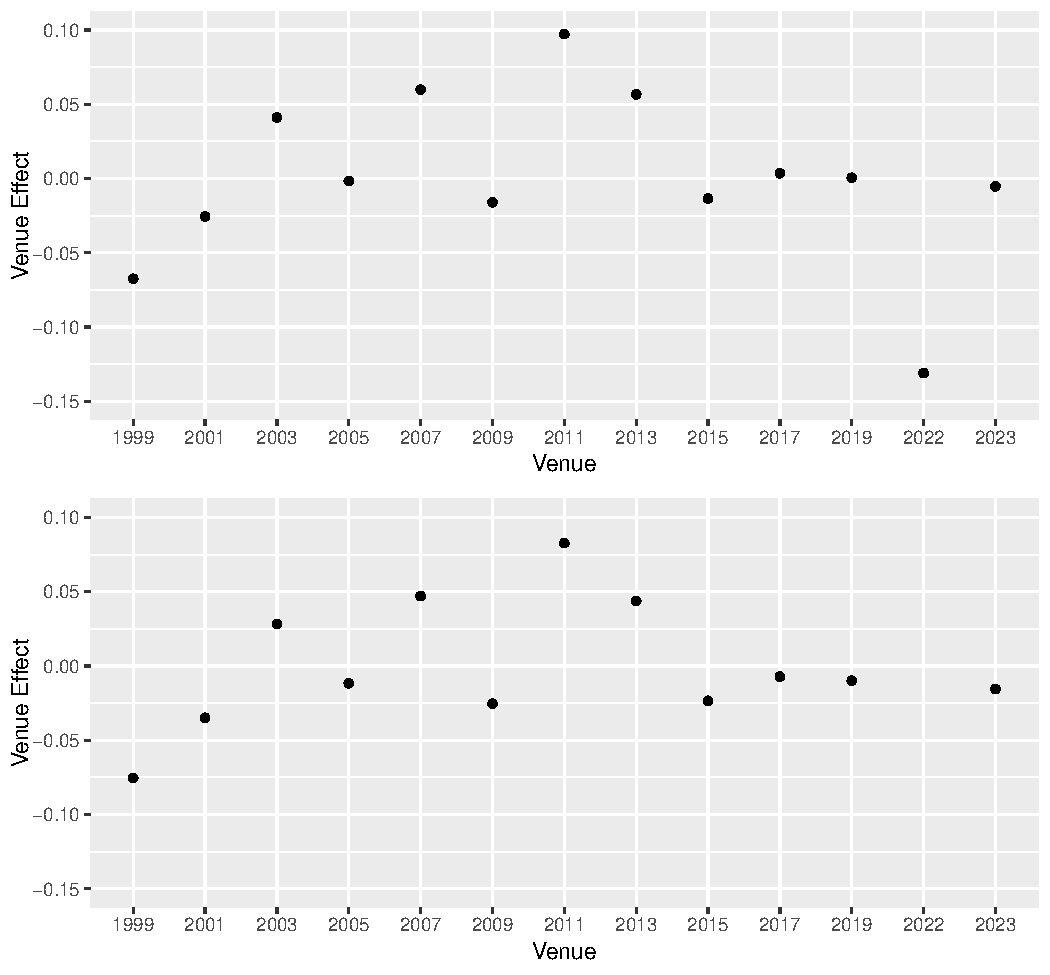
\includegraphics{ComparisonOfVenueEffects}
  \caption{The venue effects from 1999 to 2023 estimated from the GLMM for the
    data including 2022 (top) and excluding 2022 (bottom).}
  \label{fig:VenueEffects}
\end{figure}


Figure~\ref{fig:VenueEffects} further illustrates the venue effect from 1999 to
2023 based on the full GLMM both with and without 2022.  The temporal patterns
of the two sets of effects look very similar, except that the positive effects
estimated with 2022 included have higher magnitude than those estimated without
2022, which compensates the negative effect of the 2022 with a large magnitude.
Both plots agree to some extent with the pattern of the boxplots in
Figure~\ref{fig:Boxplot}. The mismatch is due to the heat effect, since the venue
effect only captures a smaller part of the variation than the heat effect as
evident from their standard deviations. It is possible to calculate the extremity
of the 2022 heat effect as we know that the mean of the heat effects is $0$,
the standard deviation is $0.42$ as given by Table~\ref{tab:Gamma_parameters},
and the estimate of the 2022 heat effect is $-0.93$. We find the tail probability
to be $0.0128$ indicating there is a low chance of observing a venue effect as
extreme as 2022.


\begin{table}
  \centering
  \caption{Probabilities of observing reaction times less than threshold 0.08,
  0.09, and 0.10 seconds based on the two effect model.}
  \begin{tabular}{c c c c} 
   \toprule
   Data Set & Threshold 0.08 & Threshold 0.09 & Threshold 0.10  \\ 
   \midrule
   Excluding 2022 & $1.10\cdot10^{-5}$ & $2.34\cdot10^{-4}$ &  $2.36\cdot10^{-3}$  \\ 
   Including 2022 & $1.71\cdot10^{-5}$ & $3.01\cdot10^{-4}$ & $2.90\cdot10^{-3}$ \\
   \bottomrule
  \end{tabular}
  \label{tab:Sim_probability}
\end{table}
\of{table has been updated}

The GLMM with both venue and heat random effects helps us to assess how extreme
a reaction time below a given threshold is. The probability of observing a reaction
time below a threshold, assuming no intentional false starts, can be
approximated by generating a large number of realizations from the fitted
GLMM. We used 10 millions realizations in the analysis. 
Table~\ref{tab:Sim_probability} summarizes the estimated probabilities of
observing a reaction time below 0.08, 0.09, and 0.10 seconds under two different
scenarios: one excluding and the other including data from 2022. Apparently,
excluding 2022 lowered the probability of observing a fast reaction time, but
the difference is not big in magnitude. For example, the probability for
seeing a reaction time below 0.10 seconds changes from $2.36\cdot 10^{-3}$ to
$2.90\cdot 10^{-3}$ when 2022 is included. These values correspond to one in
every 344 starts and 423 starts, respectively. The table shows that changing the
reaction time barrier from 0.1 seconds to 0.08 seconds drastically reduces the
chance of observing a reaction time below the barrier, from one in roughly every
283 starts to one in every 58480 starts using data with 2022 included. The
results substantiates the recommendations by \citet{komi2009iaaf}.


\begin{table}
  \centering
  \caption{Suggested reaction time barriers based on tail probabilities.}
  \begin{tabular}{c c c} 
   \toprule
   Data Set & Tail probability  $10^{-3}$ & Tail probability $10^{-4}$ \\ 
   \midrule
   Excluding 2022 & $0.096$ & $0.087$ \\ 
   Including 2022 & $0.095$ & $0.086$ \\
   \bottomrule
  \end{tabular}
  \label{tab:Sim_time}
\end{table}
\of{table has been updated}

Utilizing the same model, we can subtly shift our interpretation to determine a
suitable reaction time barrier based on the probability of observing a time
below said barrier. Including 2022 data, a reaction time barrier of 0.092
seconds is warranted to maintain a 0.1\% chance of observing an illicitly fast
reaction time, as delineated in Table~\ref{tab:Sim_time}. This calculation can
be replicated for various probability levels; for instance, a probability of
0.0001 (equating to one disqualification per 10,000 starts) necessitates a
reaction time barrier of 0.083 seconds. The exclusion of 2022 data, which
inherently lowers the probability of observing a swift reaction time, mandates a
less lenient reaction time barrier when calculated based on probability, albeit
without a substantial difference in magnitude.


\section{Discussion}\label{sec:concludingremarks}

We set out to answer two questions: were athletes who competed at the 2022 World
Track and Field Championships faster than at other races and is the 0.1 second
reaction time barrier fair.  In regards to the first question, we do believe
that athletes were faster than in comparable meets.  Ideally we would like to
be able to draw data from a central database containing every World Athletics
certified meet which we could use to reference athlete's reaction times.
Unfortunately that is not available at the moment and nearly all of the results
listed on the World Athletics website do not contain reaction times.  The results
of the study could have been stronger if we had been able to look at every race
that athletes like Devon Allen ran in 2022 and analyzed his results at the World
Championship against many other data points.

In addition to the GLMM results results presented above women, the supplementary
file contains results about the women's GLMM results.  We fit a generalized
gamma model to womens 100 meter dash and 100 meter hurdle data from 1999 to 2023
to determine an appropriate reaction time barrier.  We chose to separate these
two studies due to publications suggesting reaction time differences in men and
women.

\of{I think there are some good ideas in these 2 paragraphs but need help
integrating them. Prof Schifano can you help with this?}

The uniformity of the reaction time barrier for both men and women is
perplexing, especially in light of numerous studies that suggest a divergence in
their respective reaction times \citep[e.g.,][]{lipps2011implications,
  babicc2009reaction, panoutsakopoulos2020gender}. These authors posit that
World Athletics may be overlooking inherent gender differences by establishing
an equal reaction time barrier. If gender disparities do exist and 0.1 seconds
is deemed a fair threshold for women, it logically follows that the same cannot
be deemed fair for men, given that the probability of observing sub-0.1-second
reaction times would be inherently higher. \citet{brosnan2017effects} propounds
the adoption of gender-specific reaction time barriers, a stance that appears
logical when considering biological distinctions in reaction times between
genders.


This paper aspires to offer a statistical lens through which to examine Allen's
disqualification at the 2022 World Track and Field Championships, rather than
delivering a conclusive judgment regarding potential equipment malfunction. Our
findings reveal that athletes' reaction times at the event were, in general,
faster than those recorded at other competitions, with
Table~\ref{tab:Clusrankresults} presenting multiple significant p-values that
highlight disparities in average reaction times between the 2022 Championship
and other competitions. Further, our GLMM results indicate that a reaction time
of 0.1 seconds may not be as exceptional as commonly believed. According to the
probabilities in Table~\ref{tab:Sim_time}, World Athletics might contemplate
adjusting the disqualification barrier to 0.08 seconds, thereby enabling athletes
like Allen to react more swiftly without the apprehension of
disqualification. In summary, while the results designate 2022 as an anomalous
year, Allen's time, despite resulting in disqualification, may not be
categorically extreme.


\section*{Supplementary Material}
The data and R code used for the analysis are available in a compressed file for
ease of reproducibility.

\bibliographystyle{chicago}
\bibliography{citations}


\end{document}
